\documentclass[11pt]{article}

\usepackage{multirow}
\usepackage{tabularx}
\usepackage{longtable}
\usepackage[sorting=none, backend=bibtex]{biblatex}
\usepackage[pdftex]{graphicx} 
\usepackage{amsmath}
\usepackage{amsfonts}
\usepackage{listings}
\usepackage{xcolor}
\usepackage{appendix}
\usepackage{pdfpages}
\usepackage[colorinlistoftodos, textwidth=\marginparwidth]{todonotes}

\usepackage{todonotes}


\lstset{
    frame=single,
    breaklines=true,
    postbreak=\raisebox{0ex}[0ex][0ex]{\ensuremath{\color{red}\hookrightarrow\space}}
}

\newcommand{\overbar}[1]{\mkern 1.5mu\overline{\mkern-1.5mu#1\mkern-1.5mu}\mkern 1.5mu}
\newcommand{\mbi}[1]{\textbf{\emph{#1}}}

\addbibresource{../docs/refs.bib}

\begin{document}

\author{Guilherme Aramizo Ribeiro}
\title{Visual Servoing for Power Grid Interconnection}
\maketitle

\listoftodos

\begin{abstract}
    ...
\end{abstract}

\section{Introduction}
    
    \subsection{Objective}
        Project's goal \todo[inline]{something}
        
        Requirements and Constraints
        
    \subsection{Hardware Setup}
        \begin{itemize}
        \item USB camera (ELP 2.1mm 120 def Field of View USB camera);
        \item Trossen WidowX Robotic Arm;
        \item Male connector compatible to gripper;
        \item Female connector with visual markers.
        \end{itemize}

\section{Background}

    This section provides a brief overview of subjects related to visual servoing for the power grid project. Initially it describes the topic of robotic manipulation, which involves inverse kinematics solution and the command interface to Trossen WidowX manipulator. Later it explores computer vision, like camera calibration, image acquisition parameters and tracking algorithms. Finally the visual servoing theory is reviewed, combining the two fields. \todo{add something here}

    \subsection{Robotic Manipulator}
    % serial manipulator, placement of coordinate frames, end-effector dk, Euler parameter conversion, nonlinear solution
        Serial robotic manipulators are systems designed to move a tool of interest (or end-effector) arbitrarily in space. And this system is a chain of segments connected through actuated joints, being generally revolute joints. The present section will define the kinematic description of a serial manipulator and explain a method to solve the inverse kinematics problem.
        
        \begin{figure}[h]
        \centering
        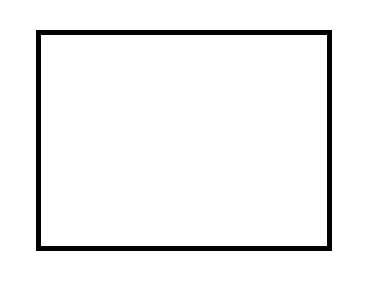
\includegraphics[width=0.35\linewidth]{img/sample}
        \caption{Coordinate frame definition on a serial manipulator}
        \label{fig:robot}
        \end{figure}
        
        When selecting a robot to a certain task, three parameters are generally observed: the number of degrees of freedom (DOF), its workspace and the maximum payload. The DOF is the number of active joints there is in the kinematic chain. If all joints act the end-effector motion independently, the DOF is simply the number of end-effector mobility. The workspace, which is the space through which the tool can translate to. Finally, the payload is the maximum weight is can manipulate with the end-effector. It is usually represented as the weight at worst case scenario position or given as a curve with weight vs distance to the base.
        
        The Inverse Kinematics (IK) Problem is the calculation of the joint angles to move the end-effector in a certain position and orientation. The basic process for this solution is
        
        \begin{enumerate}
        \item Define a coordinate frame $F_i$ in each robot segment;
        \item Calculate the rotation matrix and translation from frame $F_i$ to frame $F_{i+1}$ as a function of joint angle $q_i$;
        \item Represent the end-effector position and orientation in the base frame $F_0$;
        \item Solve the nonlinear system of equations for the joint angles, given the end-effector coordinates.
        \end{enumerate}
        
        For the kinematic description of the robot, this paper defines a vector defined in a coordinate frame $F_i$ as $^i\mbi{r}$, the orientation and translation of frame $F_i$ in respect to frame $F_j$ as $^j\mbi{R}_i$ and $^j\mbi{t}_i$, respectively. And the composition of both the translation and rotation as the 4D transformation matrix $^j\mbi{T}_i$ such that
        
        \begin{equation}
        ^j\mbi{r} =\ ^j\mbi{R}_i\ ^i\mbi{r} +\ ^j\mbi{t}_i
        \label{eq:rottrans}
        \end{equation}
        
        Equation \ref{eq:rottrans} can be represented as a single matrix multiplication if the vector is augmented by a unitary element. 
        
        \begin{equation}
            \left( 
            \begin{array}{c}
                ^j\mbi{r} \\
                1
            \end{array} 
            \right)
            = \left(
            \begin{array}{c|c}
                ^j\mbi{R}_i & ^j\mbi{t}_i \\ \hline
                0\ 0\ 0 & 1
            \end{array}
            \right)
            \left(
            \begin{array}{c}
                ^i\mbi{r} \\
                1
            \end{array}
            \right)
        \end{equation}
        
        \begin{equation}
            ^j\overbar{\mbi{r}} =\ ^j\mbi{T}_i\ ^i\overbar{\mbi{r}}
        \end{equation}

        For the kinematic representation of a $n$ DOF robot, it's convenient to define a coordinate frame $F_i$ to the axis of rotation of each of the $i^{th}$ joint, from the base to the end-effector. Therefore, a vector in the end-effector frame $F_n$ is represented on the base frame $F_0$ as

        \begin{align}
        ^j\overbar{\mbi{r}} & = (^0\mbi{T}_1\ ^1\mbi{T}_2\ ...\ ^{n-1}\mbi{T}_n)\ ^n\overbar{\mbi{r}} \\
        & =\ ^0\mbi{T}_n\ ^n\overbar{\mbi{r}}
        \end{align}
        
        The matrix $^0\mbi{T}_n$ represents the pose of the end-effector in respect to the base frame as a function of the joint angles. If an Euler angle rotation of Z-Y-X $(\psi, \theta, \phi)$ is considered, the Cartesian position and orientation are extracted from the transformation matrix as
        
        \begin{align}
        x & =\ ^0\mbi{T}_n(1,4) \\
        y & =\ ^0\mbi{T}_n(2,4) \\
        z & =\ ^0\mbi{T}_n(3,4) \\
        \psi & = atan2(^0\mbi{T}_n(2,1), ^0\mbi{T}_n(1,1)) \\
        \theta & = asin(-^0\mbi{T}_n(3,1)) \\
        \phi & = atan2(^0\mbi{T}_n(3,2), ^0\mbi{T}_n(3,3))
        \end{align}
        
        Once the Forward Kinematics Equations are defined, the Inverse Kinematics Problem is solved by numerically computing the joint angles for a desired end-effector coordinates. Numerical solvers like Python Scipy's \textbf{Optimization} package or MATLAB's \textbf{fsolve} function can be used in this stage.
        
        If the robot has a mobility less than 6, only a subset of the equations can be solved. The selection of equations depends on the particularities of the robot construction.
        
        Another interesting derivation of the Forward Kinematics Equations is the Jacobian matrix, that relates the rate of change of the end-effector coordinates and the joint angles. If $f_i$ is the $i_{th}$ end-effector coordinate and $q_j$ is the $j_{th}$ joint angle, the Jacobian is calculated as
      
        \begin{equation}
            \mathbf J = \frac{d\mathbf f}{d\mathbf q} =
            \begin{bmatrix}
            \dfrac{\partial \mathbf{f}}{\partial q_1} \cdots \dfrac{\partial \mathbf{f}}{\partial q_n} \end{bmatrix}
            = \begin{bmatrix}
            \dfrac{\partial f_1}{\partial q_1} \cdots \dfrac{\partial f_1}{\partial q_n}\\
            \vdots \ddots \vdots\\
            \dfrac{\partial f_m}{\partial q_1} \cdots \dfrac{\partial f_m}{\partial q_n} \end{bmatrix}
        \end{equation}
        
    \subsection{Computer Vision}
    % Definition, camera-lenses parameters, calibration, camera settings
        Computer vision uses image processing to reproduce the human ability of vision. The performance of these algorithms depends on a good camera-lenses selection, camera settings and calibration procedures. This section will give an overview of these subjects.
        
        Colour is our perception of the light reflected from a scene. The source of the light, or illuminant, emits electro-magnetic radiation at a wavelength of $ 400 $ to $ 700\ nm $ and as it clashes against the scene surface, some frequency components are absorved and others are reflected, depending on the material's reflectivity properties.
        
        Saturation: Purity of a color, or how 
        
        % camera-lenses parameters and settings: camera models, resolution, frame rate, lenses (FOV), distortion
        
        
        % calibration: focal point, distortion fix (3d ray to 2d map), intrinsic and extrinsic calibration
        
        Optimizing Image Quality: frame rate, auto-exposition time, bright/contrast etc
        
        Calibration
        
        Lens distortion on wide FOV cameras
    
    \subsection{Visual Servoing}
    % Control schemes, camera positioning, tracked features
        Visual Servoing is the use of computer vision as a feedback to a manipulator action. This section describes the most common control schemes, the camera placing architecture and options of tracked image features.
        
        Control schemes: 
        
        Camera 
    
        Trajectory planning. Keeping target in field of view (FOV)
        
        Camera placement, perspective error (Gripper to camera transformation estimation algorithm) ---------- Extrinsic camera calibration (hand-eye calibration)


\section{Methodology}
    This section describes the necessary steps to deploy the visual servoing system. It includes the initial setup procedures, like source dependencies installation, creation of configuration files and camera calibration. Following, it describes the control algorithm and a performance test. 
    
    \begin{figure}[h]
    \centering
    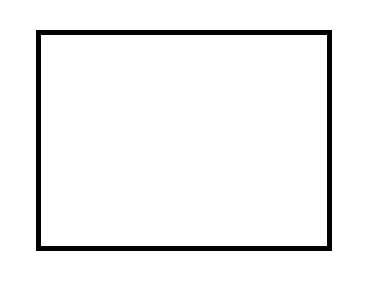
\includegraphics[width=0.35\linewidth]{img/sample}
    \caption{Diagram of program arquitecture, including the data flow and configuration files' dependencies}
    \label{fig:setup}
    \end{figure}
    
    \subsubsection{Dependencies Installation}
        The visual servoing system relies on a ROS Indigo Installation and several ROS packages and libraries. 
        
        For the robotic control and interface it uses the Python numerical library Scipy for the IK calculations, a Python binding for the Kinematics and Dynamics Library (KDL) to perform the Forward Kinematics, the U-Robot Description Format ROS package to import a robot description file into KDL and the Arbotix ROS package to control the Dynamixel servomotors of WidowX.
        
        The computer vision component requires the USB CAM ROS package for camera interface and a ROS binding for the Alvar Augmented Reality Library.
        
        \noindent The following script carries out the installation of all the dependencies. It should be executed in a desktop running Ubuntu 14.04 LTS with a ROS Indigo installation.
        \lstinputlisting[language=bash]{../docs/commands.txt}

    \subsection{Configuring the Robotic Arm Description and Interface}
        The manipulator description and interface are defined by two different configuration files, the Unified Robot Description Format (URDF) and YAML file defining the Dynamixel servomotor network.
        
        The arm description file ...
        
        The manipulator interface file ...
    
    \subsection{Configuring the Vision System}
        The vision system requires the intrinsic and extrinsic calibration files, and the visual target description. The intrinsic calibration file defines the internal properties of the camera-lenses combination, while the extrinsic calibration file defines the position and orientation of the camera in respect to the robotic arm. Also, the target is described by visual cues using a XML file.
        
        The camera calibration ... % calib board, workspace, output parameters
        
        The AR Alvar library ... % choice of bundle tag position, xml generation
        
    \subsection{Deployment}
        
        
    \subsection{Algorithm}
        State1: Look around until target is found. Cam $^W(yaw) = (ang*sin(alf*time))$\\
        State2: centralize target. $^C(x,y) = (->0, ->0).$\\
        State3: approximate to target. $Target-Cam ^C(x,y,z) = (0,0,->z0). $\\
        State3: orbit around target. $Target ^T(pitch,yaw,dist) = (->0,->0,d0)$\\
        State5: connect $^T(pitch,yaw,dist) = (0,0,->0)$\\
        
        Pseudo-code of main ROS node (visser.py)
    
    \subsection{Performance Test}
        Describe reachable workspace (attitude included) and speed

\section{Conclusion}
    Verify if initial workspace requirements are met

    \subsection{Development Timeline}
        Table with dated problems encountered and proposed solutions
        
\printbibliography
    
\clearpage    
\appendix
\appendixpage


\section{Intrinsic Camera Calibration}
Latest version available at \cite{intCalibration}.
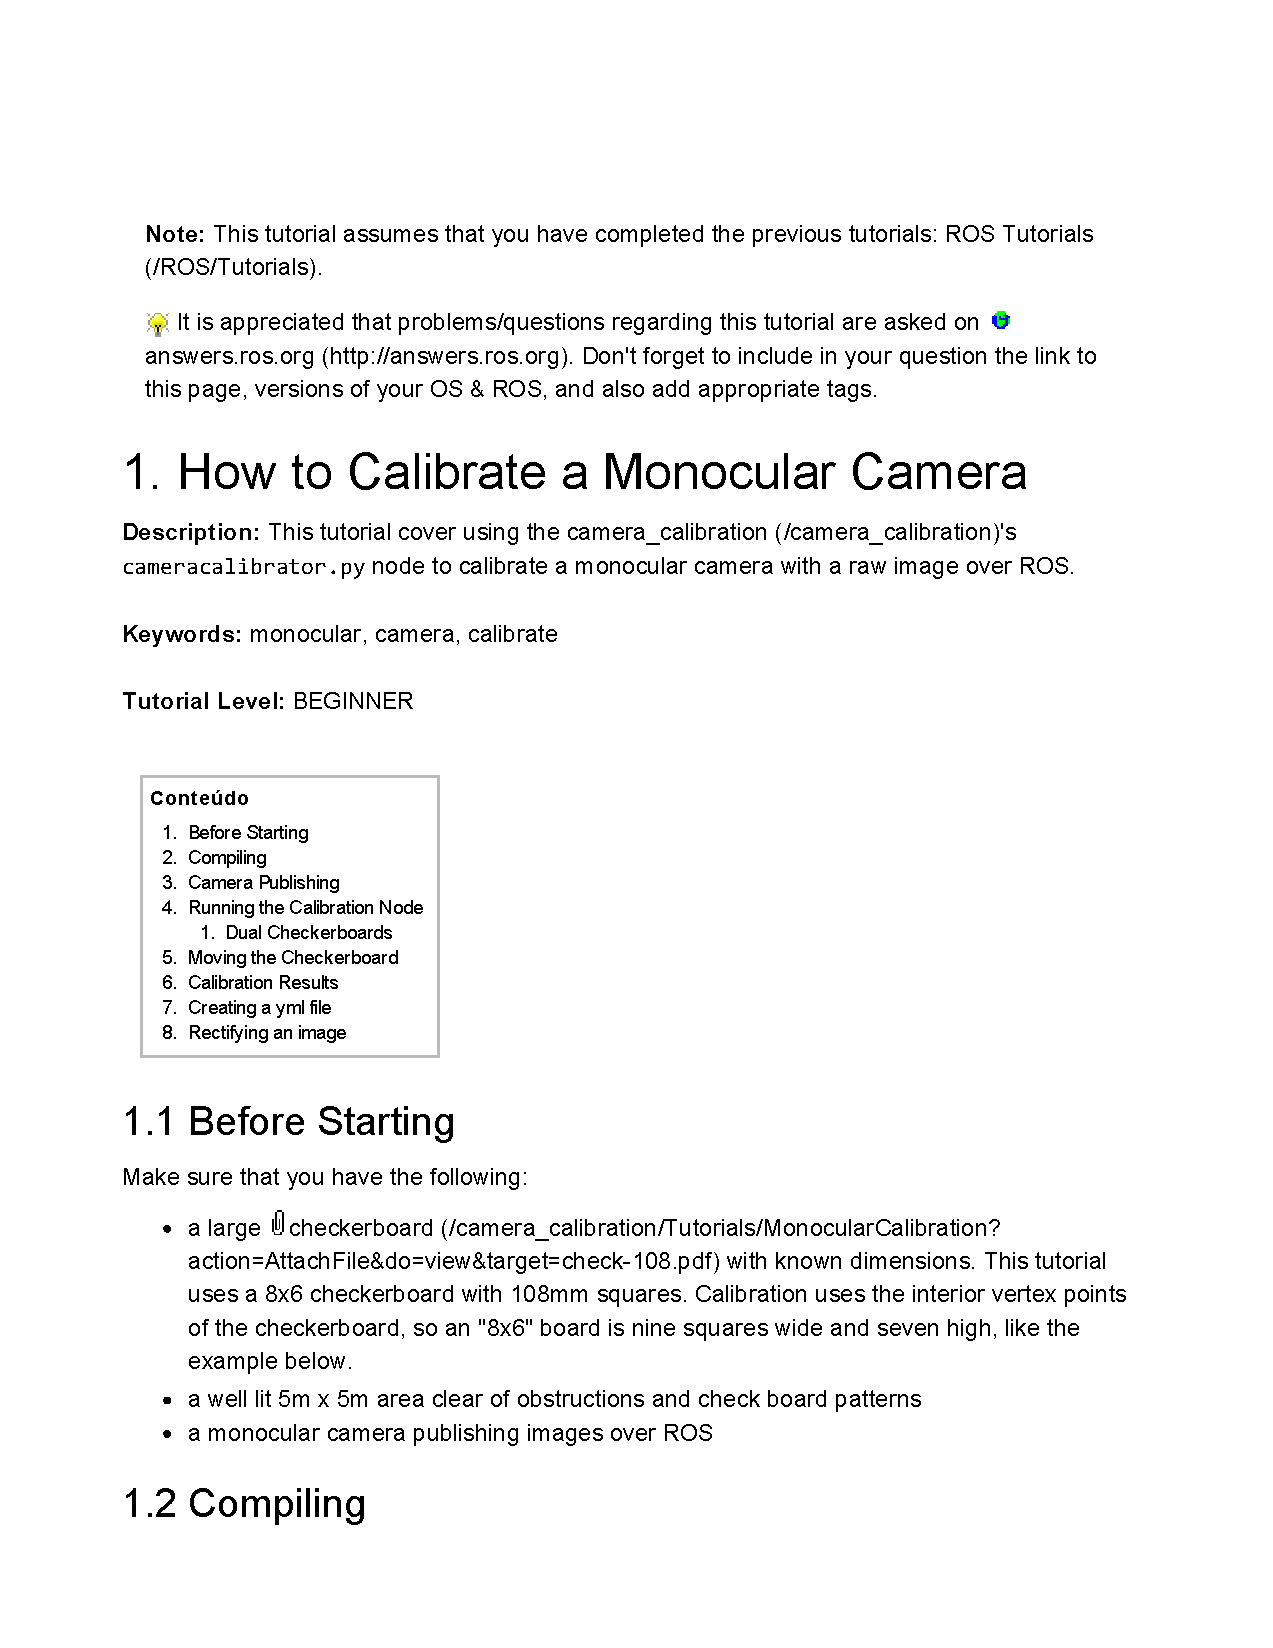
\includepdf[pages={-}]{../docs/intrinsic_calibration.pdf}

\section{Extrinsic Camera Calibration}
Latest version available at \cite{extCalibration}.
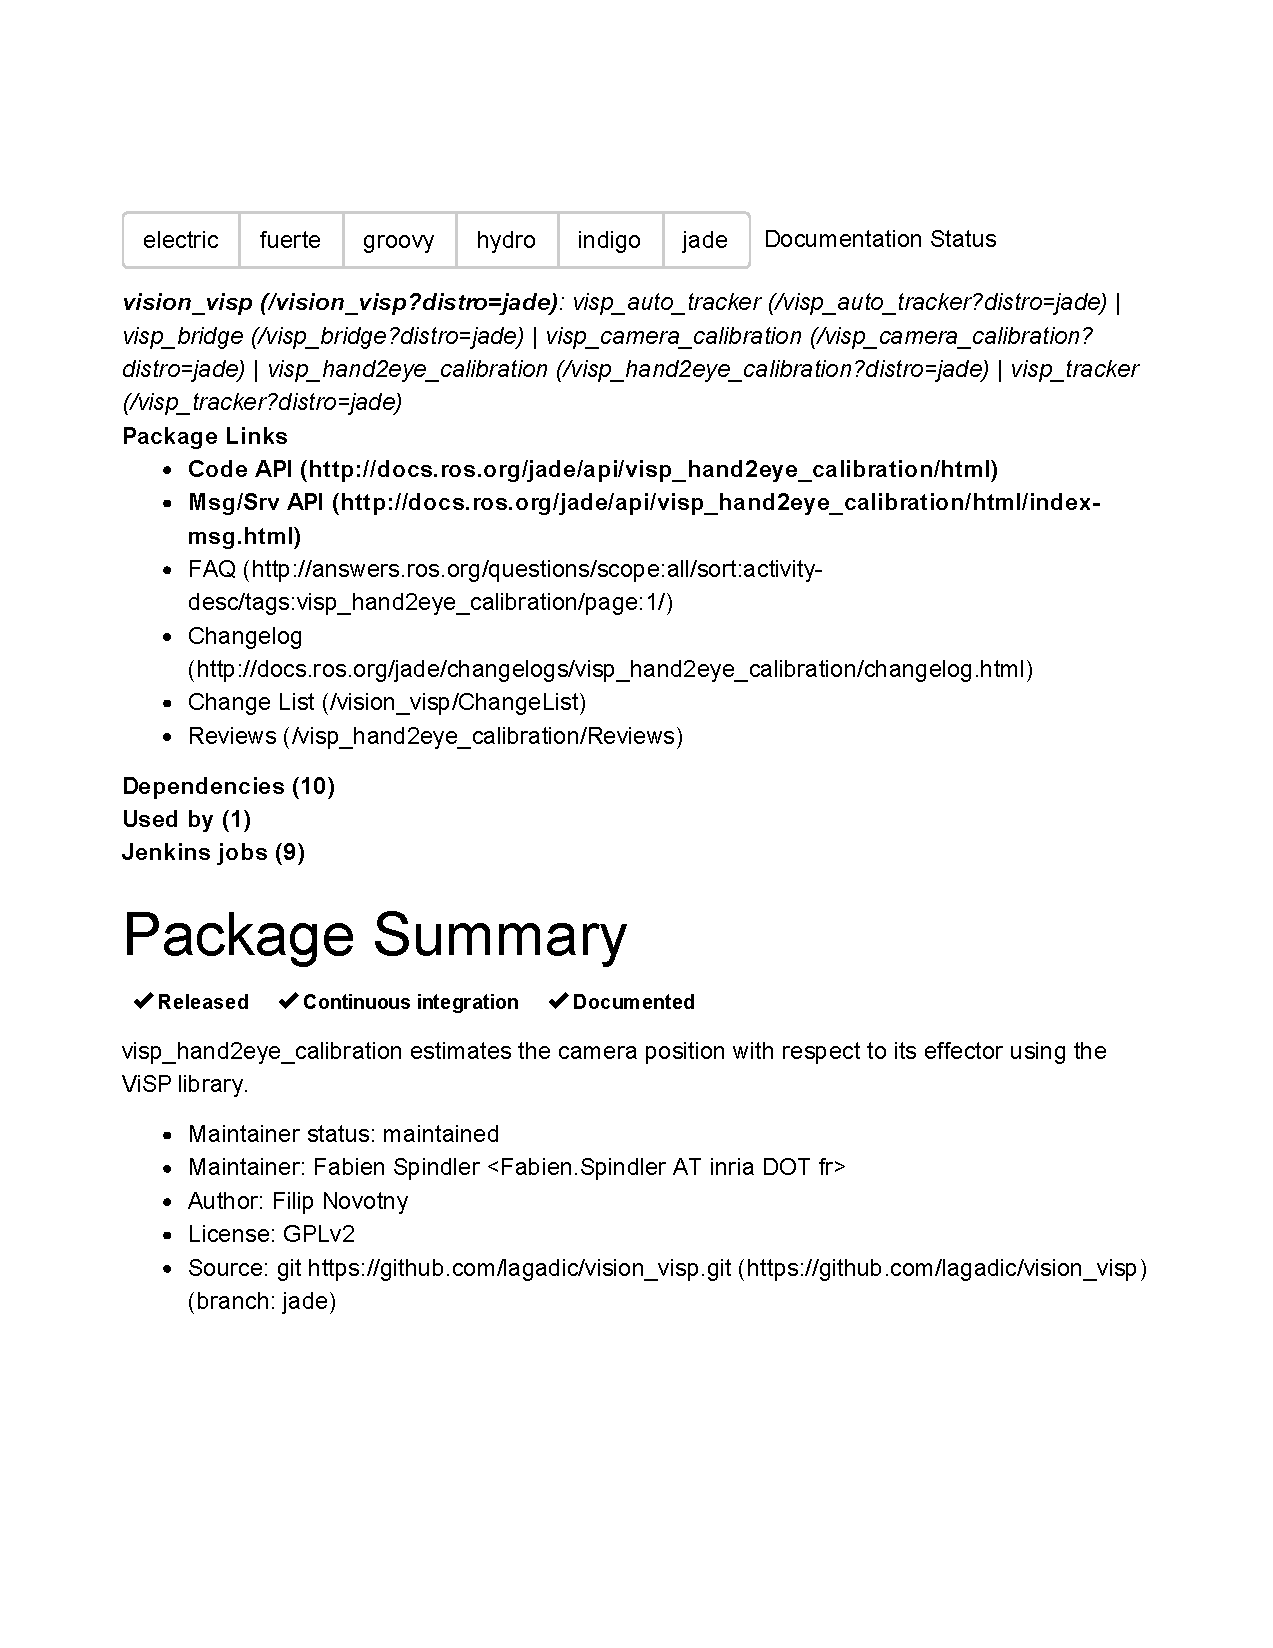
\includepdf[pages={-}]{../docs/extrinsic_calibration.pdf}

\end{document}
